\documentclass[11pt]{article}

\usepackage[utf8]{inputenc}
\usepackage[T1]{fontenc}
\usepackage{amsmath, amssymb, amsthm, amsfonts}
\usepackage{mathtools}
\usepackage{bm}
\usepackage{booktabs}
\usepackage{graphicx}
\usepackage{xcolor}
\usepackage{hyperref}
\usepackage[margin=1in]{geometry}
\usepackage{caption}
\usepackage{subcaption}
\usepackage{float}
\usepackage{enumitem}

\hypersetup{colorlinks=true, linkcolor=blue!60!black, citecolor=blue!60!black, urlcolor=blue!60!black}

\theoremstyle{definition}
\newtheorem{remark}{Remark}

% ---- Lightweight algorithm environment ----
\newcounter{algcounter}
\newenvironment{algobox}[1]{%
  \refstepcounter{algcounter}%
  \par\medskip\noindent\hrule\vspace{2pt}%
  \noindent\textbf{Algorithm \thealgcounter:} \textit{#1}\par\vspace{2pt}\hrule\vspace{4pt}%
  \begingroup\small
  \begin{tabbing}\quad\=\quad\=\quad\=\quad\=\quad\=\kill
}{%
  \end{tabbing}\endgroup\vspace{-8pt}\hrule\medskip
}

\newcommand{\R}{\mathbb{R}}
\newcommand{\E}{\mathbb{E}}
\newcommand{\Sv}{\boldsymbol{\Sigma}}
\newcommand{\Phiv}{\boldsymbol{\Phi}}
\newcommand{\Mv}{\boldsymbol{M}}
\newcommand{\Jv}{\boldsymbol{J}}
\newcommand{\Kv}{\boldsymbol{K}}
\newcommand{\diag}{\operatorname{diag}}
\newcommand{\logsumexp}{\operatorname{logsumexp}}

\title{Residual-Aware Clustering for Piecewise Dynamical Surrogates:\\[0.3em]\large From Physics Simulation to Strategic Planning}
\author{Lorenzo Tomaz\\AE Studio}
\date{}

\begin{document}
\maketitle

\begin{abstract}
Building tractable surrogates of complex systems is a prerequisite for planning, sensitivity analysis, and decision-making. We address the partition problem---how to divide a system's state space into regions where simple local models are accurate---by framing piecewise dynamical modeling as a Cluster-Weighted Model. Unlike standard clustering, which partitions by geometry alone, our approach assigns observations to clusters based on both geometric proximity and local-model prediction quality. The resulting partition follows linearizability contours rather than density contours.

We validate the framework on classical dynamical systems with known ground truth. On the Lorenz attractor, partitioned local Extended Dynamic Mode Decomposition (EDMD) models achieve $8.8\times$ lower one-step error than a single unpartitioned EDMD model at the same polynomial degree. On the damped pendulum, a physics-constrained Taylor variant matches the accuracy of an unpartitioned EDMD model with 42 times fewer parameters.

We then apply the same framework to a black-box planning task: a transformer trained on tic-tac-toe. Treating the transformer's output trajectory as a discrete dynamical system, we fit piecewise polynomial surrogates in logit space. In head-to-head play across 200 rounds at each of 11 temperature settings, a quadratic surrogate significantly outperforms the transformer at 10 settings. The surrogate generalizes to out-of-distribution board states where the transformer's sequence memorization fails---demonstrating that piecewise dynamical surrogates can serve as tractable world models for planning, not just for physics simulation.
\end{abstract}

%% ============================================================================
\section{Introduction}
%% ============================================================================

Many systems of interest---physical, biological, computational---can be queried but not easily analyzed. A chaotic attractor can be simulated forward but its sensitivity to perturbations is hard to characterize. A neural network can produce outputs but its internal reasoning is opaque. In both cases, one wants a \textbf{surrogate}: a simpler model that is cheap to evaluate, amenable to analysis (eigenvalues, sensitivity, rollouts, what-if scenarios), and faithful enough to the original system to be useful for prediction or planning.

A natural approach is \textbf{piecewise modeling}: partition the state space into $N$ regions, each with a simple local model $L_k(x)$. A single global linear model $f(x)\approx Ax+b$ works only near a fixed point; a piecewise collection of linear models can cover an attractor, a phase portrait, or a decision landscape. The key question is: \emph{how should the partition be chosen?}

Standard clustering (e.g., Gaussian Mixture Models, GMM~\cite{mclachlan2000gmm}) partitions by geometric density, ignoring the system's dynamics. A region with high density but high curvature is a poor region for a local model. The partition should follow \emph{linearizability contours}---boundaries where the local model's accuracy degrades---not density contours.

\subsection{Approach: Cluster-Weighted Models for Dynamics}

We frame piecewise dynamical modeling as a \textbf{Cluster-Weighted Model} (CWM)~\cite{gershenfeld1997,ingrassia2012,ingrassia2014}. A CWM models the joint density $p(x,y)=\sum_k\pi_k\,p(x|k)\,p(y|x,k)$, where $x$ is the system state and $y$ is the system output (a velocity, a next state, or any observable). Each cluster contributes two factors: a \emph{proximity} term measuring geometric fit, and a \emph{residual} term measuring prediction quality. Points are assigned to the cluster that best explains both where they are and what the system does there.

This framework is general. When $y=\dot{x}$ (a velocity field), it recovers piecewise modeling of ODEs. When $y=x_{t+1}$ (a next state), it models discrete-time dynamics. When $y$ is the output of a black-box system (e.g., logits from a neural network), it models input-output dynamics without requiring access to the system's internals.

\subsection{Contributions}

\begin{enumerate}[leftmargin=*,itemsep=2pt]
  \item We formulate piecewise dynamical modeling as a CWM and provide two local-model parameterizations: a physics-constrained Taylor variant (zero free parameters per cluster) and a discrete Koopman operator per cluster (data-only, no integration required).
  \item On classical dynamical systems with known ground truth (Lorenz attractor, damped pendulum), we demonstrate that residual-aware clustering significantly outperforms geometry-only clustering (GMM), and that local discrete Extended Dynamic Mode Decomposition (EDMD~\cite{williams2015data}) achieves $8.8\times$ lower error than a single unpartitioned EDMD model on the Lorenz system ($p<0.001$, 10 seeds).
  \item We apply the same framework to a \textbf{black-box planning task}: a transformer trained on tic-tac-toe. Treating the transformer's output trajectory as a discrete dynamical system, we fit piecewise surrogates in logit space. In head-to-head play, a quadratic surrogate significantly outperforms the transformer at 10 of 11 temperature settings, demonstrating that CWM-based surrogates can generalize to out-of-distribution inputs where the original system fails. We present this as an initial proof of concept; the game's simplicity is a limitation we discuss explicitly.
\end{enumerate}

\subsection{Paper Organization}

Section~\ref{sec:related} positions this work relative to piecewise system identification, Koopman methods, world models, and strategic reasoning. Section~\ref{sec:method} presents the CWM framework, the EM algorithm, and the two local-model variants. Section~\ref{sec:known} validates the method on systems with known ground truth (Lorenz, pendulum). Section~\ref{sec:planning} applies it to black-box planning on tic-tac-toe. Section~\ref{sec:discussion} analyzes why the surrogate outperforms the original system and discusses limitations and future directions.

%% ============================================================================
\section{Related Work}\label{sec:related}
%% ============================================================================

\textbf{Piecewise affine system identification.} Ferrari-Trecate et al.~\cite{ferrari2003clustering} and Paoletti et al.~\cite{paoletti2007identification} identify piecewise affine models via two-stage procedures: cluster the data, then fit local models. Our CWM formulation performs both simultaneously---the clustering is informed by the dynamics, not just geometry. Recent work on Gaussian Process Switching Linear Dynamical Systems (gpSLDS)~\cite{gpslds2024} achieves smooth interpolation between locally linear regimes; our approach uses hard-partition EM with Bayesian pruning, trading smoothness for interpretability of the cluster boundaries.

\textbf{Koopman operator theory and EDMD.} The Koopman operator~\cite{brunton2022modern} lifts nonlinear dynamics into a linear framework via observables. Dynamic Mode Decomposition (DMD)~\cite{schmid2010dmd,tu2014dmd} approximates the Koopman operator from data; Extended DMD (EDMD)~\cite{williams2015data} generalizes this to richer observable bases such as polynomials. Deep Koopman methods~\cite{lusch2018deep} learn the observable basis end-to-end with neural networks. Koopman Model Predictive Control~\cite{korda2018koopman} uses the linear Koopman representation for real-time control, and Koopman-Assisted Reinforcement Learning (KARL)~\cite{karl2024} constructs a ``Koopman tensor'' parameterized by control actions for planning in lifted coordinates. MetaKoopman~\cite{metakoopman2025} uses Bayesian meta-learning with Normal-Inverse-Wishart priors over Koopman operators---the same prior family we employ for cluster parameters. All of these fit a \emph{single} model; we fit \emph{local} models per cluster, which handles systems that are not globally linearizable in any finite basis.

\textbf{World models and surrogate-based planning.} World models serve as surrogates for real environments, enabling planners like Model Predictive Control or Monte Carlo Tree Search to query the model at inference time~\cite{worldmodelsurvey2025}. Code World Models~\cite{codeworldmodels2024} use LLMs to generate Python simulators for model-based RL. Neural MPC surrogates~\cite{neuralmpc2024} replace physics simulators with neural networks for real-time control. These approaches use opaque neural surrogates; our piecewise models are interpretable---each cluster's local operator can be inspected, its eigenvalues computed, its sensitivity analyzed.

\textbf{Transformers as dynamical systems.} Recent work analyzes transformers through the lens of dynamical systems. The residual stream can be viewed as a discrete-time trajectory evolving through layers~\cite{mechanalysis2024}. Transformer Dynamics~\cite{transformerdynamics2025} applies neuroscientific tools to analyze rotational dynamics in hidden states. The CFDRA framework~\cite{tomaz2025cfdra} shows that each RoPE attention head is algebraically equivalent to a bank of damped harmonic oscillators. These works \emph{analyze} transformer dynamics; we go further and \emph{build surrogates} of those dynamics for planning.

\textbf{Strategic reasoning in games.} Game Theory meets LLMs~\cite{gtllm2025} surveys how LLMs perform on game-theoretic tasks. GTBench~\cite{gtbench2024} evaluates strategic reasoning capabilities. Game of Thoughts~\cite{gameofthoughts2025} uses iterative reasoning for game-theoretic planning. These approaches evaluate or improve reasoning via prompting and search. Our approach is fundamentally different: we extract the dynamics of the system's outputs, learn a piecewise surrogate, and plan through the surrogate's dynamics.

\textbf{Hierarchical Mixtures of Experts and Cluster-Weighted Models.} Jordan and Jacobs~\cite{jordan1994hme} introduced Hierarchical Mixtures of Experts (HME), using EM-based gating to route inputs to local expert models based on prediction quality---the conceptual foundation for input-dependent mixture models. Jacobs et al.~\cite{jacobs1991adaptive} proposed the original adaptive mixtures of local experts. Gershenfeld~\cite{gershenfeld1997,gershenfeld1999nature} formalized this into Cluster-Weighted Models (CWMs) for time-series analysis, explicitly modeling the joint density of input and output. Ingrassia et al.~\cite{ingrassia2012,ingrassia2014} developed the Linear Gaussian CWM, and Punzo~\cite{punzo2014poly} extended CWMs to polynomial local models. Our work extends this lineage to dynamical systems with physics-constrained (Taylor) and Koopman-theoretic (EDMD) local models, and demonstrates their use as plannable surrogates of black-box systems.

\textbf{Switching dynamical systems.} Fox et al.~\cite{fox2011bayesian} develop Bayesian nonparametric switching linear dynamical systems; Ghahramani and Hinton~\cite{ghahramani2000variational} introduce variational learning for switching state-space models. These approaches use \emph{temporal} regime switching---the mode changes over time. Our method uses \emph{spatial} phase-space partitioning---the mode depends on where the system is in state space. The two approaches are complementary.

%% ============================================================================
\section{Method}\label{sec:method}
%% ============================================================================

\subsection{Problem Statement}

Given observations $\{(x_i, y_i)\}_{i=1}^P$ from a system where $y_i = F(x_i)$ for some unknown or expensive function $F\colon\R^d\to\R^m$, find a piecewise model consisting of $N$ clusters with centers $c_k$, covariances $\Sv_k$, and local models $L_k$, such that $L_k(x)\approx F(x)$ within the region associated with cluster $k$.

The state $x$ may be a position in phase space ($y=\dot{x}$, the velocity field), a current state ($y=x_{t+1}$, discrete dynamics), or any system input ($y$ = system output). The method treats $(x, y)$ pairs uniformly.

\subsection{Generative Model}

We model the joint density of state and output as a Cluster-Weighted Model:
\begin{equation}
  p(x_i, y_i) = \sum_{k=1}^N \pi_k \underbrace{\mathcal{N}(x_i;\, c_k,\, \Sv_k)}_{\text{proximity}} \cdot \underbrace{\mathcal{N}(y_i - L_k(x_i);\, 0,\, \sigma_k^2 I)}_{\text{residual quality}}.
\label{eq:cwm}
\end{equation}

The \textbf{proximity factor} $\mathcal{N}(x_i; c_k, \Sv_k)$ is the standard Gaussian mixture component, measuring geometric fit. The \textbf{residual factor} $\mathcal{N}(y_i - L_k(x_i); 0, \sigma_k^2 I)$ measures how accurately the local model $L_k$ predicts the output at $x_i$. The per-cluster residual scale $\sigma_k^2$ is learned during EM, allowing each cluster to adapt its prediction tolerance. Mixing weights $\pi_k$ are subject to a sparse Dirichlet prior $\pi\sim\mathrm{Dir}(\alpha_0\mathbf{1})$ with $\alpha_0<1$, encouraging automatic pruning of unnecessary clusters.

The joint criterion ensures that points are assigned to clusters where the local model is accurate, not merely where they are geometrically close. A region of high density but high curvature receives low residual likelihood, forcing the partition to respect the dynamics. The generative process is illustrated in Figure~\ref{fig:generative}.

\begin{figure}[htbp]
\centering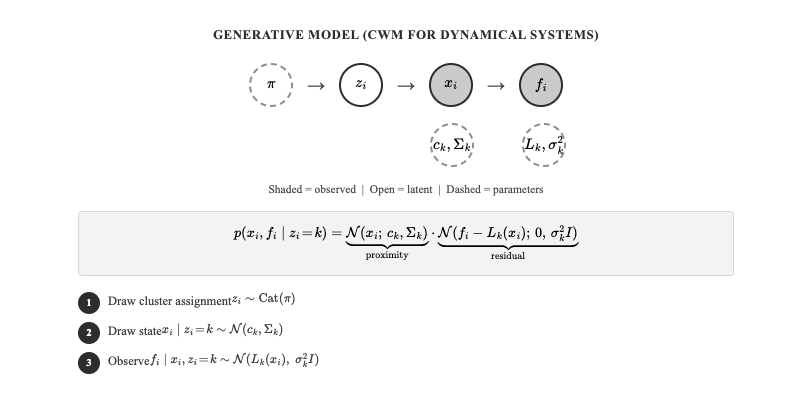
\includegraphics[width=0.85\textwidth]{figures/01_generative_model.png}
\caption{Generative model: each observation $(x_i, y_i)$ is generated by drawing a cluster $z_i\sim\mathrm{Cat}(\pi)$, then drawing $x_i$ from the proximity model and $y_i$ from the local model plus noise.}
\label{fig:generative}
\end{figure}

\subsection{EM Algorithm}

We fit the model by Expectation-Maximization, alternating between soft cluster assignments (E-step) and parameter updates (M-step).

\textbf{E-step.} Compute responsibilities:
\begin{equation}
  r_{ik} = \frac{\pi_k\,\mathcal{N}(x_i; c_k, \Sv_k)\,\mathcal{N}(y_i - L_k(x_i); 0, \sigma_k^2 I)}{\sum_{j=1}^N \pi_j\,\mathcal{N}(x_i; c_j, \Sv_j)\,\mathcal{N}(y_i - L_j(x_i); 0, \sigma_j^2 I)}.
\label{eq:estep}
\end{equation}
The E-step is identical across all local-model variants---it depends on the local model only through its predictions $L_k(x_i)$.

\textbf{M-step.} Update all parameters using the responsibilities as soft weights:
\begin{itemize}[leftmargin=*,itemsep=1pt]
  \item \textbf{Centers} $c_k$: weighted mean with NIW posterior regularization.
  \item \textbf{Covariances} $\Sv_k$: NIW posterior mode from the weighted scatter matrix.
  \item \textbf{Local models} $L_k$: variant-specific (see Section~\ref{sec:variants}).
  \item \textbf{Mixing weights} $\pi_k$: Dirichlet posterior mode $\hat{\pi}_k \propto R_k + \alpha_0 - 1$, where $R_k = \sum_i r_{ik}$.
  \item \textbf{Residual variance} $\sigma_k^2$: estimated from weighted prediction residuals.
\end{itemize}

The full EM iteration is shown in Figure~\ref{fig:em-loop}, and the responsibility computation is detailed in Figure~\ref{fig:responsibility}.

\textbf{Dead cluster pruning.} When $R_k < 1$ (effective cluster mass below one point), the cluster is removed. With $\alpha_0 < 1$, the Dirichlet prior drives unused clusters toward zero weight, enabling automatic model selection: start with $N$ larger than needed and let the prior prune.

\begin{figure}[htbp]
\centering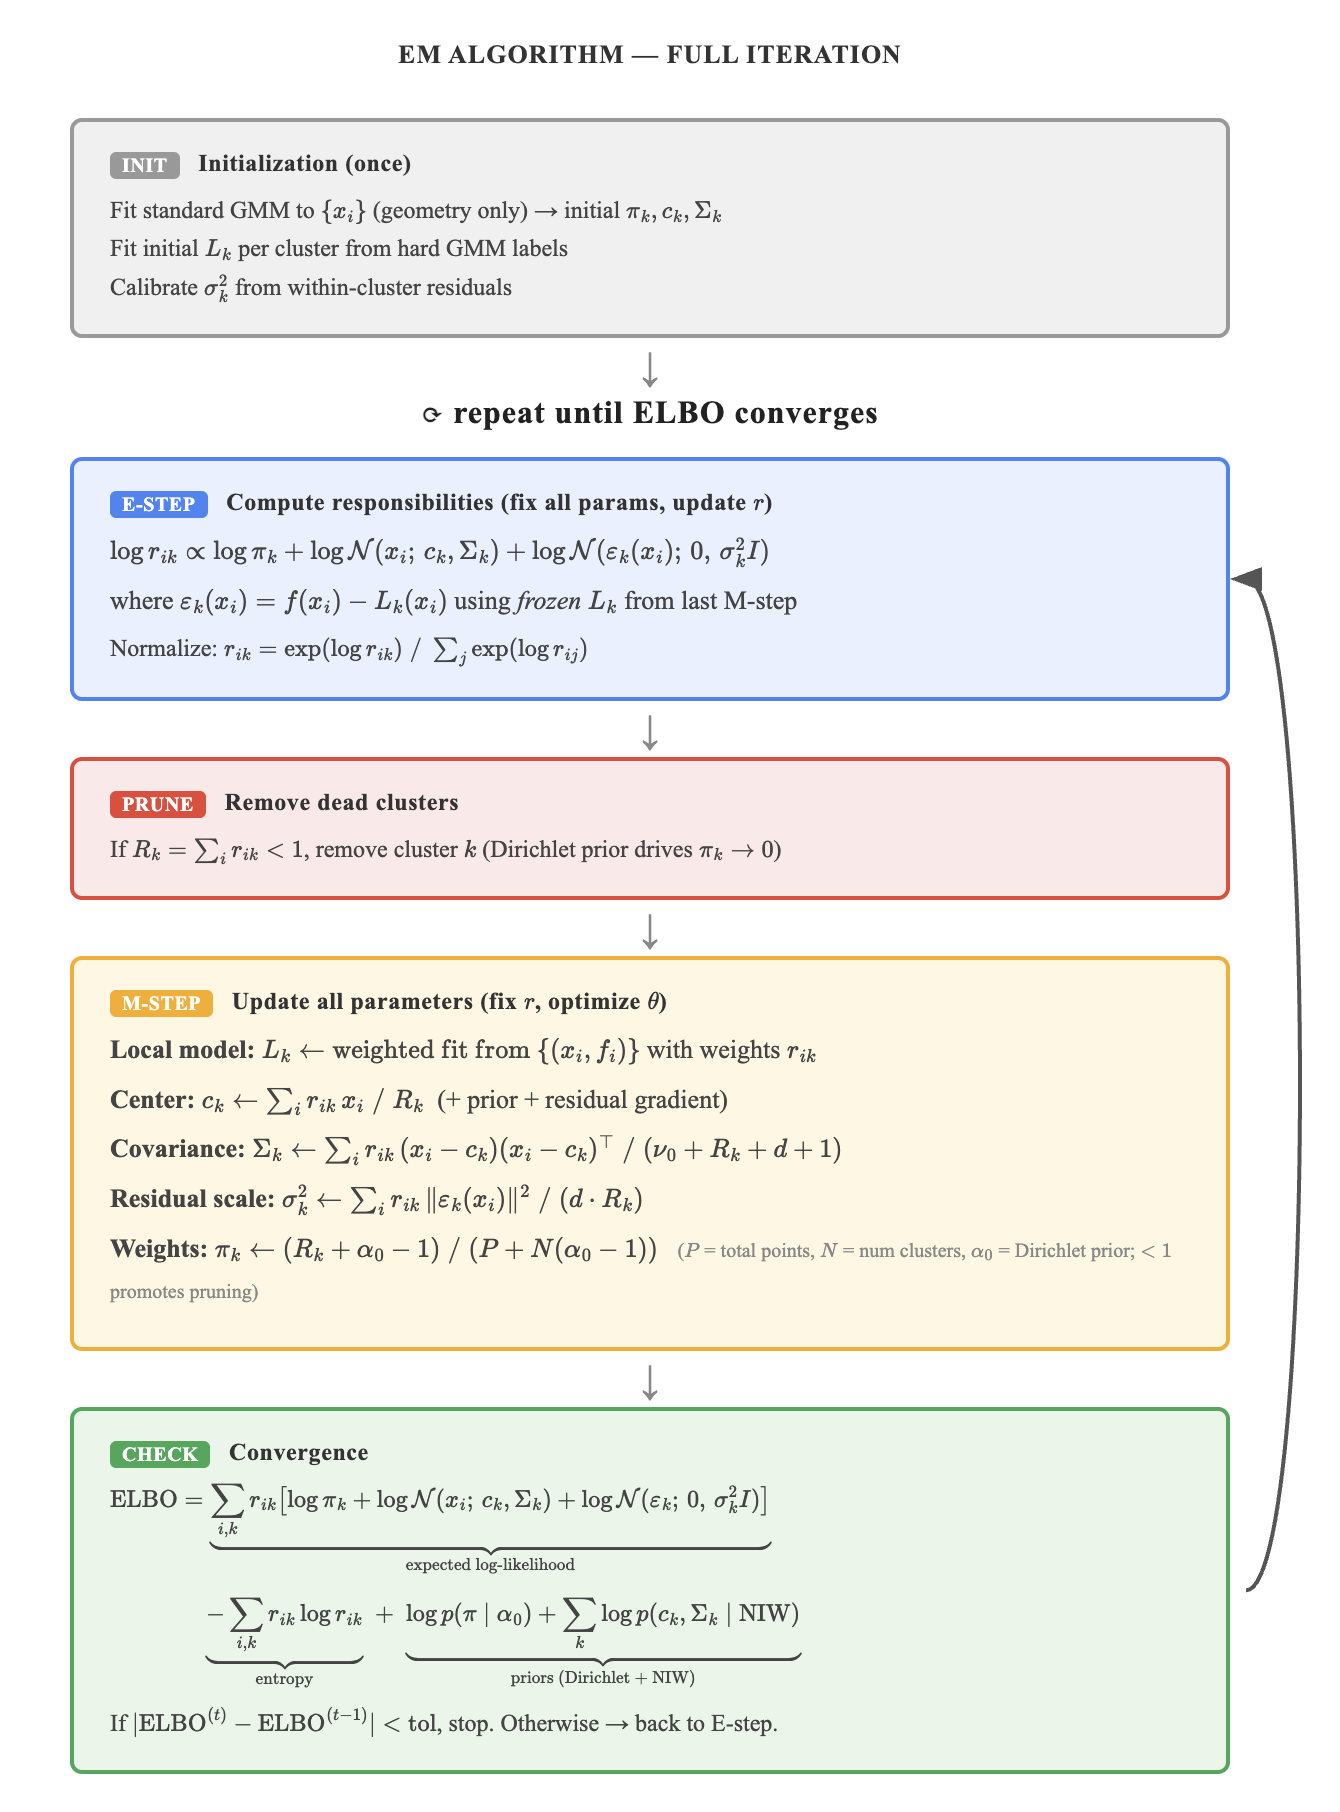
\includegraphics[width=0.88\textwidth]{figures/02_em_loop.png}
\caption{Full EM iteration. The E-step computes soft assignments using frozen parameters; the M-step updates all parameters using fixed responsibilities. Dead clusters are pruned when $R_k < 1$.}
\label{fig:em-loop}
\end{figure}

\begin{figure}[htbp]
\centering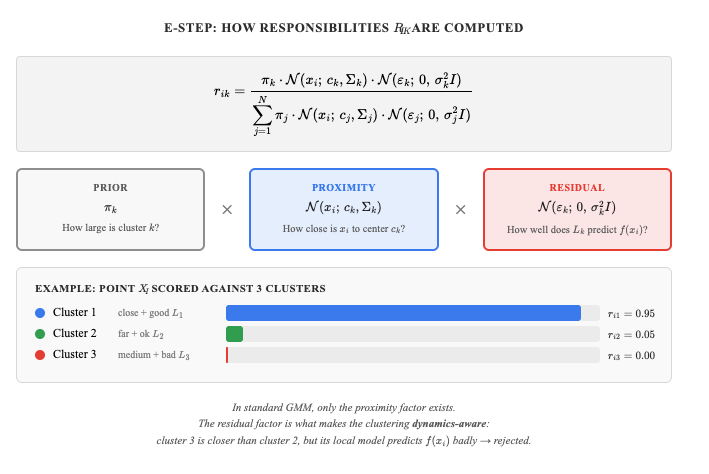
\includegraphics[width=0.85\textwidth]{figures/04_responsibility.png}
\caption{Responsibility computation. Each point is scored against every cluster by three factors: prior weight, proximity, and residual quality. The residual factor can override proximity---a geometrically close cluster with poor predictions gets low responsibility.}
\label{fig:responsibility}
\end{figure}

\subsection{Bayesian Priors and Model Selection}

For cluster parameters $(c_k, \Sv_k)$ we use a Normal-Inverse-Wishart (NIW) prior: $\Sv_k\sim\mathcal{IW}(\Psi_0, \nu_0)$, $c_k|\Sv_k\sim\mathcal{N}(\mu_0, \Sv_k/\kappa_0)$. The proximity marginal is available in closed form; the residual factor is evaluated at the converged point estimate $\hat{c}_k$ (a plug-in approximation adequate when $R_k$ is large).

The Evidence Lower Bound (ELBO) decomposes as:
\begin{equation}
  \mathcal{L} = \underbrace{\sum_{ik} r_{ik}\log\pi_k}_{\text{assignment}} + \underbrace{\sum_{ik} r_{ik}\log\mathcal{N}(x_i; c_k, \Sv_k)}_{\text{proximity}} + \underbrace{\sum_{ik} r_{ik}\log\mathcal{N}(\varepsilon_{ik}; 0, \sigma_k^2 I)}_{\text{residual}} + H[q] + \log p(\theta)
\end{equation}
where $\varepsilon_{ik} = y_i - L_k(x_i)$, $H[q]$ is the entropy of the variational distribution, and $\log p(\theta)$ includes the Dirichlet and NIW priors. The ELBO is guaranteed non-decreasing across EM iterations (with a mild GEM approximation for the Taylor-analytic variant).

\subsection{Local-Model Variants}\label{sec:variants}

The CWM framework is agnostic to the form of the local model $L_k$. Any function that maps an input $x$ to a predicted output $y$ can serve as a local model, provided it can be fit from weighted data during the M-step. We present two variants that cover the most common settings: one that exploits analytical knowledge of the system, and one that works from data alone.

\subsubsection{Variant A: Taylor-Analytic}

Consider a smooth dynamical system $\dot{x} = f(x)$ where the function $f$ and its Jacobian $\Jv(x) = \partial f / \partial x$ are known analytically. By Taylor's theorem, the vector field near any point $c$ is well approximated by its first-order expansion:
\begin{equation}
  f(x) \approx f(c) + \Jv(c)(x - c) + O(\|x - c\|^2).
\end{equation}
This approximation is accurate within a neighborhood whose radius depends on the curvature of $f$---the higher the curvature, the smaller the region where the linear approximation holds. This is precisely the motivation for partitioning: by placing cluster centers $c_k$ throughout the state space, each cluster's Taylor expansion only needs to be accurate within its own region.

The local model for cluster $k$ is:
\begin{equation}
  L_k(x) = f(c_k) + \Jv(c_k)(x - c_k).
\end{equation}
This variant has \textbf{zero free local parameters}---$f(c_k)$ and $\Jv(c_k)$ are completely determined by the center $c_k$ and the known physics. During the M-step, after the center is updated, we simply re-evaluate $f$ and $\Jv$ at the new center. This re-tying is a Generalized EM (GEM) step rather than a pure coordinate-ascent update, but empirically the ELBO remains monotone.

The Taylor-analytic variant is maximally parameter-efficient: all the model's expressiveness comes from the partition (choosing where to place centers), not from fitting local parameters. When the physics are known, this is the optimal choice.

\subsubsection{Variant B: Local Discrete EDMD}

When the system's dynamics are unknown---we can observe consecutive states $(x_t, x_{t+1})$ but have no analytical expression for $f$---we need a data-driven approach.

The key idea from Koopman operator theory~\cite{brunton2022modern} is that a nonlinear dynamical system can be represented as a linear system in a higher-dimensional space of observables. Given a set of basis functions $\Phiv(u)$, the evolution of these observables is approximately linear:
\begin{equation}
  \Phiv(x_{t+1}) \approx \Kv \cdot \Phiv(x_t),
\end{equation}
where $\Kv \in \R^{M \times M}$ is the discrete Koopman matrix and $M$ is the number of basis functions. The choice of $\Phiv$ is flexible: monomials, radial basis functions, Fourier features, or learned representations can all serve as the observable basis. In this work we use monomials up to degree $p$, so $\Phiv(u) = [1, u_1, \ldots, u_d, u_1^2, u_1 u_2, \ldots]$ with $M = \binom{d+p}{p}$ terms, though the framework applies to any choice of basis. The state prediction is obtained by extracting the first $d$ non-constant entries from the lifted prediction: $\hat{x}_{t+1} = [\Kv \cdot \Phiv(x_t)]_{1:d}$.

A single Koopman matrix fitted to the entire dataset may struggle when the dynamics vary across the state space---for instance, when different regions have qualitatively different behavior (as in the two lobes of the Lorenz attractor). Our approach fits a \textbf{separate Koopman matrix per cluster}, centered at $c_k$ (Figure~\ref{fig:lorenz-clusters} shows an example of how these cluster centers tile the Lorenz attractor):
\begin{equation}
  \hat{x}_{t+1} = c_k + [\Kv_k \cdot \Phiv(x_t - c_k)]_{1:d}.
\end{equation}
Working in centered coordinates $(x - c_k)$ ensures that the monomial basis is well-conditioned within each cluster. The matrix $\Kv_k$ is fit by weighted least squares, where the weights are the responsibilities from the E-step:
\begin{equation}
  \Kv_k = \arg\min_{\Kv} \sum_i r_{ik} \|\Phiv(x_{i,t+1} - c_k) - \Kv\cdot\Phiv(x_{i,t} - c_k)\|^2.
\end{equation}
This has a closed-form solution via the (weighted) pseudoinverse, so the M-step for each cluster is a single linear algebra operation.

The discrete EDMD variant requires no knowledge of the system's equations, no numerical integration, and no time-step parameter. It works wherever consecutive input-output pairs are available---whether the system is a differential equation sampled at discrete times, a recurrence relation, or a black-box function observed at successive steps.

\begin{table}[H]
\centering\small
\begin{tabular}{lllll}
\toprule
Variant & Params/cluster & Needs $\Jv$? & Data requirement \\
\midrule
Taylor-analytic & 0 & Yes & States + known $f, \Jv$ \\
Local disc.\ EDMD & $\binom{d+p}{p}^2$ & No & Consecutive pairs $(x_t, x_{t+1})$ \\
\bottomrule
\end{tabular}
\caption{Local-model variants. Taylor-analytic exploits physics knowledge for maximum parameter efficiency. Discrete EDMD is the data-only variant, applicable to any system with consecutive input-output pairs.}
\label{tab:variants}
\end{table}

\subsection{Prediction}

At test time, the output $y$ is unavailable, so cluster assignment uses proximity only:
\begin{equation}
  k^* = \arg\max_k\; \pi_k\,\mathcal{N}(x;\, c_k,\, \Sv_k).
\end{equation}
The local model $L_{k^*}$ then predicts. This introduces a mild distribution shift from training (where both proximity and residual quality determined assignment), but the shift is small because the EM has already aligned proximity regions with residual-quality regions. The full prediction pipeline is illustrated in Figure~\ref{fig:prediction}.

\begin{figure}[htbp]
\centering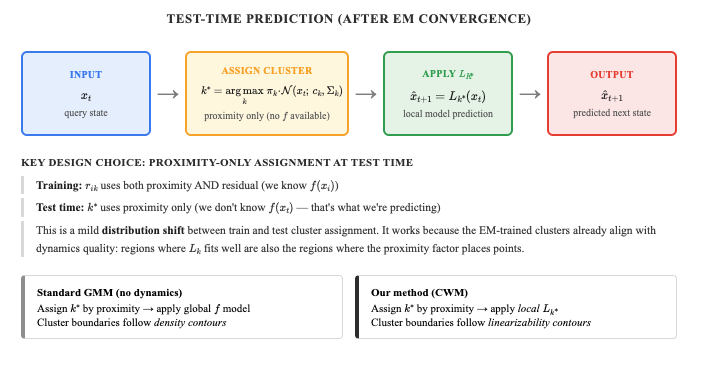
\includegraphics[width=0.9\textwidth]{figures/05_prediction.png}
\caption{Test-time prediction. Cluster assignment uses proximity only (no output available). The trained local model $L_{k^*}$ predicts the output directly.}
\label{fig:prediction}
\end{figure}

%% ============================================================================
\section{Experiments: Known Dynamical Systems}\label{sec:known}
%% ============================================================================

We first validate the method on systems with known ground truth, where prediction accuracy can be measured exactly. All results are reported as mean $\pm$ 95\% CI across 10 random seeds. Statistical significance is assessed by paired $t$-tests.

\textbf{Metrics.} \emph{One-step error} is the root mean squared error (RMSE) of the predicted next state: $\sqrt{\frac{1}{P}\sum_i \|\hat{x}_{i,t+1} - x_{i,t+1}\|^2}$, computed on the held-out test set. \emph{Relative error} (\%) normalizes this by the mean norm of the true output. \emph{Rollout error} is the Euclidean distance between the predicted and true trajectories at a fixed time horizon (5 seconds for Lorenz, 10 seconds for pendulum), starting from a test-set initial condition and iterating the surrogate model forward.

\subsection{Lorenz Attractor ($d=3$)}

The Lorenz system $(\sigma, \rho, \beta) = (10, 28, 8/3)$:
\begin{align}
  \dot{x} &= \sigma(y - x), \quad \dot{y} = x(\rho - z) - y, \quad \dot{z} = xy - \beta z. \notag
\end{align}
Data: 5000 points at $\Delta t = 0.01$; train/test split 4000/1000.

This system is polynomial---a global degree-3 monomial lift is theoretically exact. The question is whether local models with lower-degree lifts can match or exceed global accuracy.

\begin{table}[H]
\centering\small
\begin{tabular}{lcccc}
\toprule
Method & $N$ & One-step error & Rel.\ \% & Rollout @ 5s \\
\midrule
EDMD (unpart.) deg-2 (pykoopman) & 1  & $0.0205\pm0.0023$ & $2.28\pm0.44$ & --- \\
EDMD (unpart.) deg-2 (ours)      & 1  & $0.0205\pm0.0023$ & $2.28\pm0.44$ & $16.3\pm5.0$ \\
EDMD (unpart.) deg-3             & 1  & $0.0002\pm0.0000$ & $0.03\pm0.00$ & $1.9\pm1.6$ \\
\midrule
\textbf{Local EDMD deg-2, $N\!=\!5$}  & 5  & $\mathbf{0.0023\pm0.0005}$ & $\mathbf{0.26\pm0.06}$ & $\mathbf{8.5\pm3.3}$ \\
Local EDMD deg-2, $N\!=\!12$ & 12 & $0.0005\pm0.0001$ & $0.05\pm0.02$ & $2.6\pm1.6$ \\
Local EDMD deg-2, $N\!=\!50$ & 50 & $0.0004\pm0.0002$ & $0.04\pm0.02$ & $1.7\pm1.3$ \\
\midrule
Taylor-analytic, $N\!=\!5$   & 5  & $0.1801\pm0.0105$ & $19.8\pm1.9$ & $306\pm448$ \\
Taylor-analytic, $N\!=\!20$  & 20 & $0.0676\pm0.0024$ & $7.4\pm0.6$ & $21.0\pm3.8$ \\
Taylor-analytic, $N\!=\!50$  & 50 & $0.0566\pm0.0026$ & $6.2\pm0.3$ & $17.8\pm2.6$ \\
\midrule
GMM baseline, $N\!=\!5$      & 5  & $0.2738\pm0.0223$ & $29.9\pm1.7$ & diverges \\
GMM baseline, $N\!=\!50$     & 50 & $0.1128\pm0.0115$ & $12.4\pm1.7$ & diverges \\
\bottomrule
\end{tabular}
\caption{Lorenz results (mean $\pm$ 95\% CI, 10 seeds). Local EDMD at $N\!=\!5$ achieves $8.8\times$ lower error than the unpartitioned EDMD baseline at the same polynomial degree.}
\label{tab:lorenz}
\end{table}

\textbf{Partitioned EDMD beats unpartitioned EDMD.} At $N=5$ (deg-2), local EDMD achieves $0.26\pm0.06\%$ one-step error vs the unpartitioned baseline at $2.28\pm0.44\%$---an $8.8\times$ improvement ($p<0.001$). At $N=12$, it matches the unpartitioned deg-3 model ($0.05\%$ vs $0.03\%$). This demonstrates that residual-aware partitioning helps even on polynomial systems where a single EDMD model with a sufficiently high-degree lift is theoretically exact.

\textbf{Residual-aware clustering beats GMM.} Taylor-analytic outperforms GMM at every $N$ by $+34\%$ to $+50\%$ ($p<0.001$). GMM rollouts diverge at all $N$; residual-aware rollouts remain bounded from $N\geq 5$. Figure~\ref{fig:lorenz-clusters} shows how the three methods partition the attractor, and Figure~\ref{fig:lorenz-rollout} compares rollout trajectories.

\begin{figure}[htbp]
\centering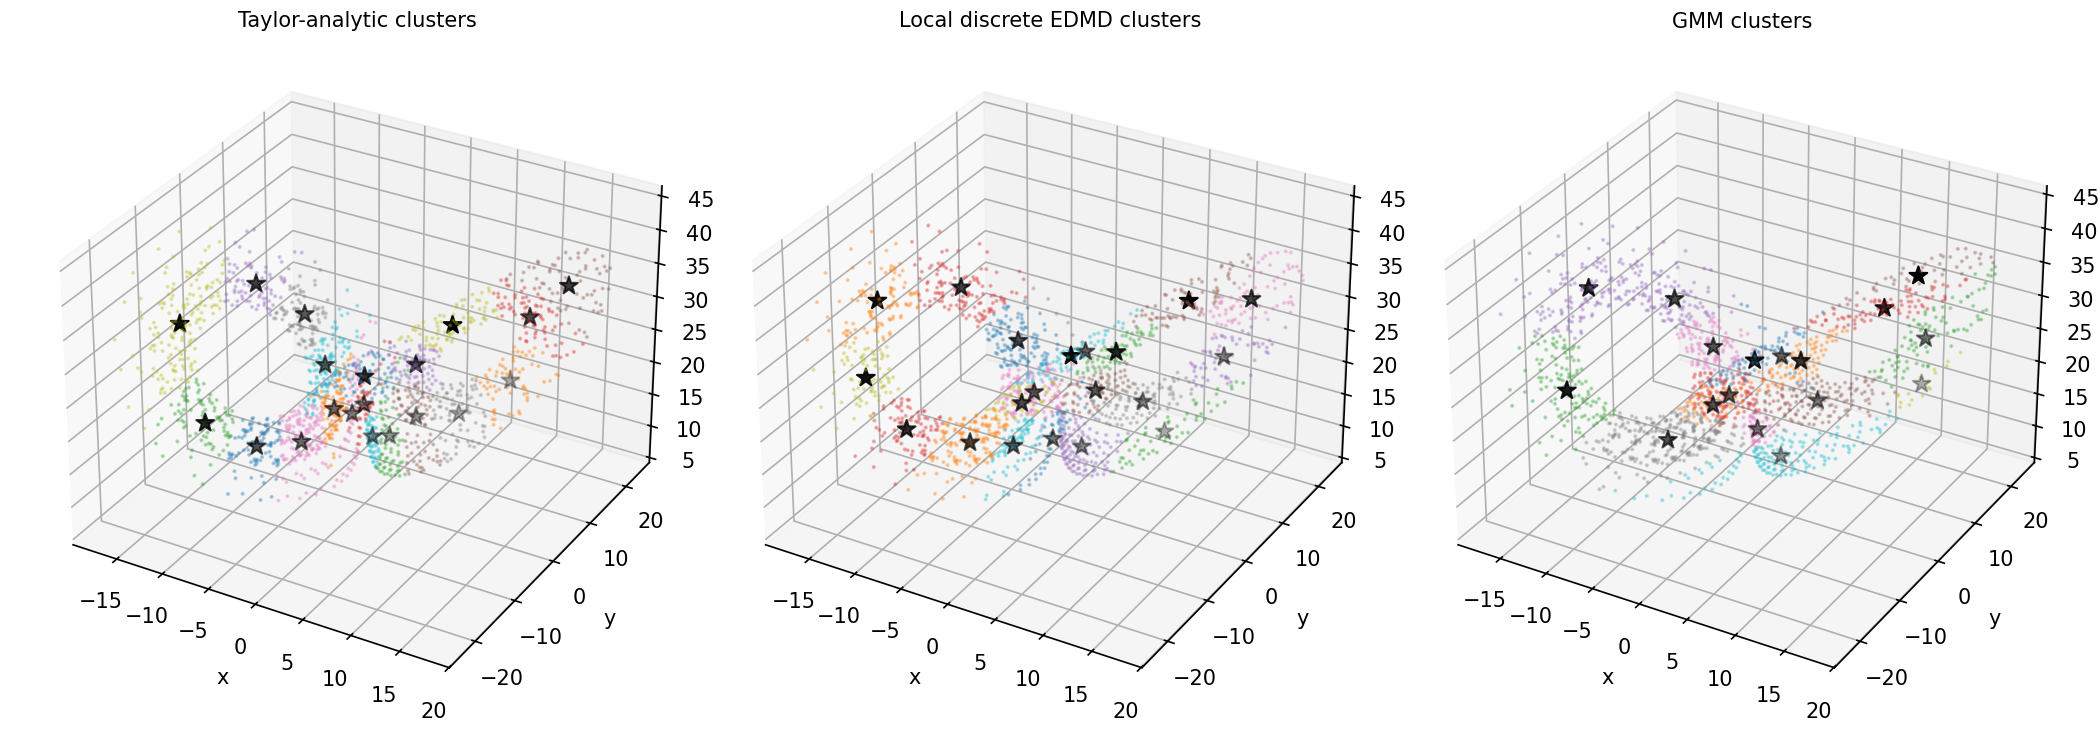
\includegraphics[width=\textwidth]{figures/lorenz_clusters_3d.png}
\caption{Lorenz attractor colored by cluster assignment (20 clusters). Left: Taylor-analytic. Center: local discrete EDMD. Right: GMM. The CWM variants produce dynamically coherent regions; GMM splits by geometry alone.}
\label{fig:lorenz-clusters}
\end{figure}

\begin{figure}[htbp]
\centering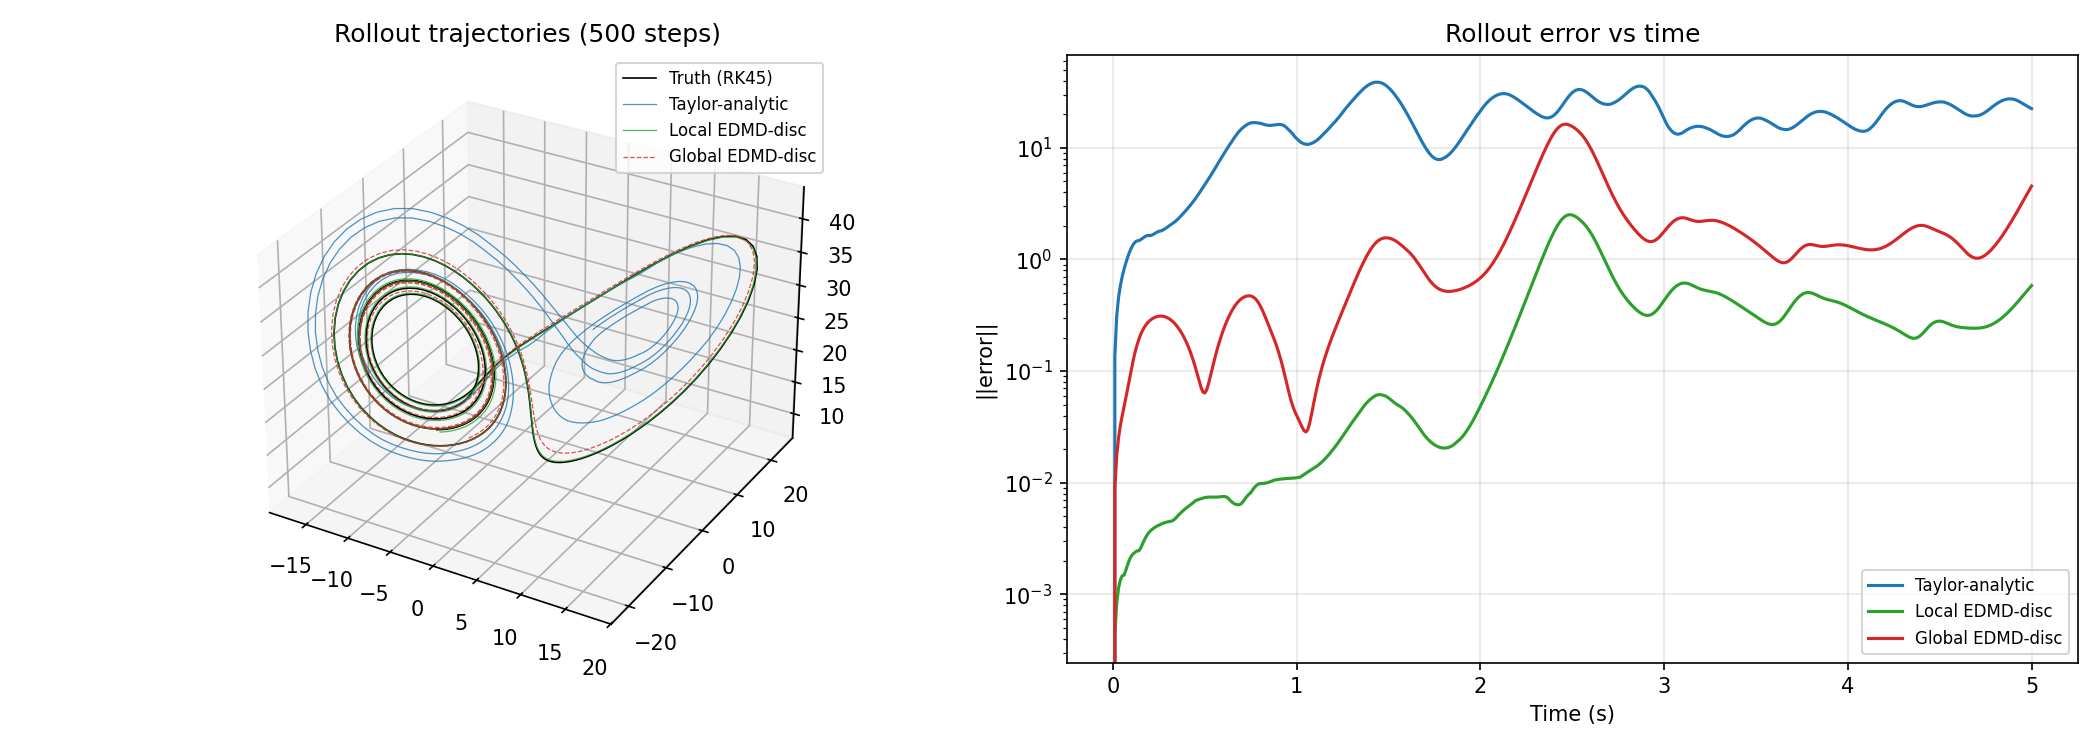
\includegraphics[width=\textwidth]{figures/lorenz_rollout_comparison.png}
\caption{Rollout trajectories from a test-set initial condition (500 steps). Local EDMD (green) tracks truth closely; unpartitioned EDMD (red) and Taylor-analytic (blue) diverge earlier.}
\label{fig:lorenz-rollout}
\end{figure}

\subsection{Damped Pendulum ($d=2$)}

The pendulum with damping $\gamma=0.2$, state $(\theta, \dot{\theta})$:
\begin{align}
  \dot{x}_1 = x_2, \quad \dot{x}_2 = -\sin(x_1) - \gamma\, x_2. \notag
\end{align}
Data: 4000 training points uniformly from $(\theta, \dot{\theta}) \in [-\pi, \pi] \times [-3, 3]$; 1000 test points.

The $\sin(\theta)$ nonlinearity has no finite polynomial representation. An unpartitioned EDMD model requires high degree to approximate it; local models sidestep this by approximating $\sin(\theta)$ within small angular ranges.

\begin{table}[H]
\centering\small
\begin{tabular}{lccccc}
\toprule
Method & $N$ & Params & One-step & Rollout @ 10s & $n$ \\
\midrule
EDMD (unpart.) deg=2 & 1 & 36   & $0.391\pm0.004$ & $0.894\pm0.009$ & 10 \\
EDMD (unpart.) deg=4 & 1 & 225  & $0.057\pm0.001$ & $0.270\pm0.007$ & 10 \\
EDMD (unpart.) deg=6 & 1 & 784  & $0.004\pm0.000$ & $0.180\pm0.000$ & 10 \\
EDMD (unpart.) deg=8 & 1 & 2025 & $0.000\pm0.000$ & $0.174\pm0.000$ & 10 \\
\textbf{Local EDMD d2, $N\!=\!2$} & 2 & \textbf{72} & $0.015\pm0.000$ & $\mathbf{0.166\pm0.005}$ & 10 \\
Local EDMD d2, $N\!=\!8$          & 8 & 288         & $0.006\pm0.001$ & $0.172\pm0.003$ & 10 \\
\textbf{Taylor-ana., $N\!=\!8$}   & 8 & \textbf{48} & $0.021\pm0.003$ & $\mathbf{0.142\pm0.006}$ & 10 \\
Taylor-ana., $N\!=\!16$           & 16 & 96          & $0.009\pm0.001$ & $0.151\pm0.004$ & 10 \\
\bottomrule
\end{tabular}
\caption{Pendulum results (mean $\pm$ 95\% CI, 10 seeds). Taylor-analytic at $N\!=\!8$ (48 params) beats the unpartitioned EDMD deg-8 baseline (2025 params) with $42\times$ fewer parameters.}
\label{tab:pendulum}
\end{table}

\textbf{Parameter efficiency.} Local EDMD deg-2 at $N=2$ (72 params) outperforms unpartitioned EDMD deg-6 (784 params): $0.166\pm0.005$ vs $0.180\pm0.000$ ($p=0.0003$)---$\sim\!11\times$ parameter efficiency.

\textbf{Physics knowledge helps.} Taylor-analytic at $N=8$ (48 params) achieves the best rollout ($0.142\pm0.006$), beating unpartitioned EDMD deg-8 (2025 params, $0.174$, $p<0.0001$) with $42\times$ fewer parameters. When the Jacobian is available, the physics-constrained variant is optimal. Phase-space rollouts are shown in Figure~\ref{fig:pendulum-rollout}.

\begin{figure}[htbp]
\centering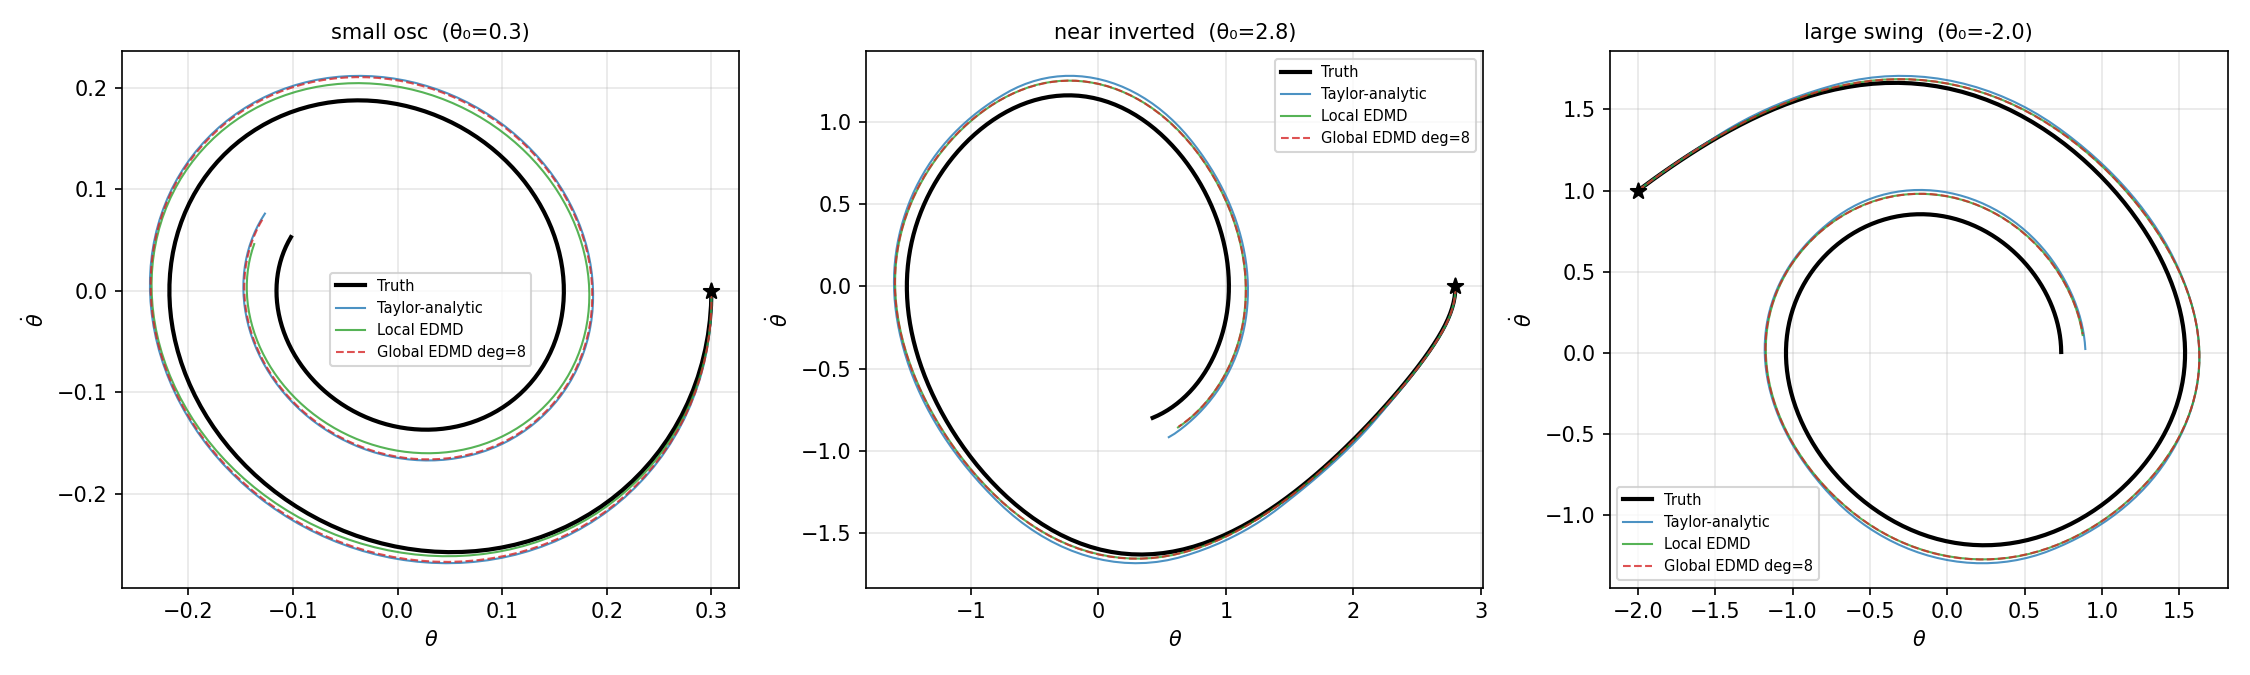
\includegraphics[width=\textwidth]{figures/pendulum_rollout_comparison.png}
\caption{Phase-space rollouts from three initial conditions (10 seconds). Local methods track truth closely; unpartitioned EDMD deg-8 is visually similar despite $14$--$42\times$ more parameters.}
\label{fig:pendulum-rollout}
\end{figure}

\subsection{Summary}

On polynomial systems (Lorenz), local Koopman partitioning improves accuracy at the same polynomial degree. On non-polynomial systems (pendulum), local models provide order-of-magnitude parameter efficiency. In both cases, residual-aware clustering strictly outperforms geometry-only clustering. These results validate the method on systems with known ground truth.

We now turn to a setting where no ground truth is available: a black-box system whose internal dynamics are unknown.

%% ============================================================================
\section{Experiments: Black-Box Strategic Planning}\label{sec:planning}
%% ============================================================================

\subsection{Task and Motivation}

We test whether the CWM framework can build useful surrogates of a system where: (i) the dynamics are unknown---the system is a black box; (ii) the goal is not just approximation but \emph{planning}---using the surrogate to make decisions; and (iii) evaluation is task performance (winning a game), not just prediction error.

We choose tic-tac-toe as a testbed: small enough to enumerate optimal play, large enough that memorization fails on out-of-distribution inputs, and well-understood game-theoretically (perfect play by both sides always draws).

\subsection{Experimental Setup}

\textbf{The black box.} A 1-layer transformer with Rotary Position Encoding (RoPE), $d_\text{model}=16$, 4 attention heads, SiLU activation, 3,424 parameters. Trained on 3,584 minimax-optimal tic-tac-toe games via cross-entropy on next-move prediction (teacher forcing). The transformer achieves 94.6\% optimal-move accuracy on held-out optimal games.

\textbf{The dynamical system.} We extract the transformer's output logit vectors at each position in a game. The logit vector $\ell_t \in \R^9$ (one entry per board cell) encodes the model's move prediction at step $t$. Consecutive logit pairs $(\ell_t, \ell_{t+1})$ define a discrete-time dynamical system in 9 dimensions. We apply the CWM framework (Eq.~\ref{eq:cwm}) to these pairs, with $x = \ell_t$ and $y = \ell_{t+1}$.

The method does not know that the logits come from a transformer, that they represent a game, or that the game is tic-tac-toe. It sees 9-dimensional input-output pairs and learns a piecewise model.

\textbf{Initial condition.} The transformer provides the initial logit $\ell_0$ by processing the [BOS] token. The surrogate predicts all subsequent logits: $\hat{\ell}_{t+1} = L_{k^*}(\ell_t)$.

\subsection{Evaluation Protocol}

We evaluate surrogates on two complementary metrics:

\textbf{Move prediction.} Given a logit from the transformer, use the surrogate to predict the next logit. Check whether $\arg\max(\hat{\ell}_{t+1})$ is a minimax-optimal move. Evaluated on 100 games (700 predictions, positions 2--8). This measures fidelity to the training distribution.

\textbf{Arena.} The transformer and surrogate play tic-tac-toe against each other for 200 rounds per temperature setting. Temperature-based sampling ($\tau > 0$) introduces move diversity by sampling from $\mathrm{softmax}(\ell / \tau)$ instead of taking $\arg\max$. Each round alternates who plays X. Statistical tests: one-sample $t$-test on the score ($+1$ = transformer win, $-1$ = surrogate win, $0$ = draw), binomial test on decisive games, Wilson 95\% CIs on win rates. This measures planning performance on out-of-distribution states.

Both metrics are needed: move prediction tests fidelity, arena tests generalization. As we will show, they measure different things.

\subsection{Surrogate Configurations}

We test polynomial surrogates at degrees 1, 2, and 3, all with 10 clusters. The degree controls expressiveness: degree 1 is linear ($M=10$ basis functions), degree 2 is quadratic ($M=55$), degree 3 is cubic ($M=220$). Higher degree means more parameters per cluster.

\begin{table}[H]
\centering\small
\begin{tabular}{lcccc}
\toprule
Surrogate & Degree & Params & Ratio vs transformer & Prediction accuracy \\
\midrule
Polynomial deg-1 & 1 & 1,920 & 0.6$\times$ & 59.0\% \\
\textbf{Polynomial deg-2} & \textbf{2} & \textbf{31,170} & \textbf{9.1$\times$} & \textbf{68.3\%} \\
Polynomial deg-3 & 3 & 484,920 & 142$\times$ & 68.9\% \\
\bottomrule
\end{tabular}
\caption{Polynomial surrogate configurations. Prediction accuracy is on minimax-optimal games.}
\label{tab:surrogate-configs}
\end{table}

\subsection{Results: Arena}

\begin{table}[H]
\centering\small
\begin{tabular}{lcccccl}
\toprule
Temp & T wins & S wins & Draws & Mean score & 95\% CI & Sig \\
\midrule
\multicolumn{7}{c}{\textit{Polynomial degree 1 (1,920 params, 0.6$\times$)}} \\
\midrule
0.0 & 0 & 100 & 100 & $-0.500$ & $[-0.569, -0.431]$ & $*$ S \\
0.1 & 93 & 47 & 60 & $+0.230$ & $[+0.118, +0.342]$ & $*$ T \\
0.2 & 105 & 58 & 37 & $+0.235$ & $[+0.114, +0.356]$ & $*$ T \\
0.3 & 99 & 60 & 41 & $+0.195$ & $[+0.074, +0.316]$ & $*$ T \\
0.4 & 98 & 65 & 37 & $+0.165$ & $[+0.042, +0.288]$ & $*$ T \\
0.5 & 103 & 54 & 43 & $+0.245$ & $[+0.127, +0.363]$ & $*$ T \\
0.6 & 107 & 43 & 50 & $+0.320$ & $[+0.208, +0.432]$ & $*$ T \\
0.7 & 99 & 52 & 49 & $+0.235$ & $[+0.119, +0.351]$ & $*$ T \\
0.8 & 88 & 64 & 48 & $+0.120$ & $[+0.000, +0.240]$ & \\
0.9 & 102 & 53 & 45 & $+0.245$ & $[+0.128, +0.362]$ & $*$ T \\
1.0 & 92 & 70 & 38 & $+0.110$ & $[-0.014, +0.234]$ & \\
\midrule
\multicolumn{7}{c}{\textit{\textbf{Polynomial degree 2 (31,170 params, 9.1$\times$)}}} \\
\midrule
0.0 & 0 & \textbf{100} & 100 & $-0.500$ & $[-0.569, -0.431]$ & $*$ \textbf{S} \\
0.1 & 10 & \textbf{94} & 96 & $-0.420$ & $[-0.501, -0.339]$ & $*$ \textbf{S} \\
0.2 & 21 & \textbf{101} & 78 & $-0.400$ & $[-0.493, -0.307]$ & $*$ \textbf{S} \\
0.3 & 36 & \textbf{119} & 45 & $-0.415$ & $[-0.523, -0.307]$ & $*$ \textbf{S} \\
0.4 & 54 & \textbf{94} & 52 & $-0.200$ & $[-0.316, -0.084]$ & $*$ \textbf{S} \\
0.5 & 57 & \textbf{96} & 47 & $-0.195$ & $[-0.313, -0.077]$ & $*$ \textbf{S} \\
0.6 & 64 & \textbf{93} & 43 & $-0.145$ & $[-0.266, -0.024]$ & $*$ \textbf{S} \\
0.7 & 65 & \textbf{95} & 40 & $-0.150$ & $[-0.273, -0.027]$ & $*$ \textbf{S} \\
0.8 & 72 & 88 & 40 & $-0.080$ & $[-0.204, +0.044]$ & \\
0.9 & 65 & \textbf{95} & 40 & $-0.150$ & $[-0.273, -0.027]$ & $*$ \textbf{S} \\
1.0 & 70 & \textbf{96} & 34 & $-0.130$ & $[-0.255, -0.005]$ & $*$ \textbf{S} \\
\midrule
\multicolumn{7}{c}{\textit{Polynomial degree 3 (484,920 params, 142$\times$)}} \\
\midrule
0.0 & 200 & 0 & 0 & $+1.000$ & --- & $*$ T \\
0.1 & 86 & 101 & 13 & $-0.075$ & $[-0.209, +0.059]$ & \\
0.2 & 104 & 77 & 19 & $+0.135$ & $[+0.004, +0.266]$ & $*$ T \\
0.3 & 93 & 92 & 15 & $+0.005$ & $[-0.129, +0.139]$ & \\
0.4 & 100 & 85 & 15 & $+0.075$ & $[-0.058, +0.208]$ & \\
0.5 & 92 & 91 & 17 & $+0.005$ & $[-0.128, +0.138]$ & \\
0.6 & 95 & 88 & 17 & $+0.035$ & $[-0.098, +0.168]$ & \\
0.7 & 108 & 80 & 12 & $+0.140$ & $[+0.007, +0.273]$ & $*$ T \\
0.8 & 100 & 88 & 12 & $+0.060$ & $[-0.074, +0.194]$ & \\
0.9 & 105 & 85 & 10 & $+0.100$ & $[-0.035, +0.235]$ & \\
1.0 & 100 & 89 & 11 & $+0.055$ & $[-0.080, +0.190]$ & \\
\bottomrule
\end{tabular}
\caption{Arena results (200 rounds per temperature). S = surrogate wins, T = transformer wins, $*$ = $p < 0.05$. The degree-2 polynomial significantly outperforms the transformer at \textbf{10 of 11} temperature settings.}
\label{tab:arena}
\end{table}

\textbf{Degree 2 is the sweet spot.} The quadratic surrogate significantly outperforms the transformer at 10 of 11 temperatures---the strongest result across all configurations. At low temperatures ($\tau \leq 0.3$), the surrogate wins 70--85\% of decisive games.

\textbf{Degree 1 is too weak.} Linear local models cannot capture the nonlinear interactions between logit dimensions. The transformer significantly outperforms the degree-1 surrogate at 8 temperatures.

\textbf{Degree 3 overfits.} Despite 142$\times$ more parameters and marginally higher prediction accuracy (68.9\% vs 68.3\%), the cubic surrogate is roughly even with the transformer in the arena. The 220$\times$220 Koopman operators (48,400 params per cluster) memorize training patterns rather than learning generalizable dynamics.

\subsection{The Prediction-Performance Gap}

\begin{table}[H]
\centering\small
\begin{tabular}{lccc}
\toprule
Surrogate & Prediction acc. & Arena: S sig.\ better & Arena: T sig.\ better \\
\midrule
Polynomial deg-1 & 59.0\% & 1 / 11 & 8 / 11 \\
\textbf{Polynomial deg-2} & \textbf{68.3\%} & \textbf{10 / 11} & \textbf{0 / 11} \\
Polynomial deg-3 & 68.9\% & 0 / 11 & 2 / 11 \\
\bottomrule
\end{tabular}
\caption{Prediction accuracy on optimal games vs.\ arena performance. Higher prediction accuracy does not imply better planning: deg-3 (68.9\%) is even, while deg-2 (68.3\%) dominates.}
\label{tab:gap}
\end{table}

Prediction accuracy measures fidelity to the training distribution (minimax-optimal games). Arena performance measures generalization to states that arise from non-optimal play (induced by temperature sampling). These are different metrics: the degree-3 surrogate memorizes optimal patterns slightly better but fails to generalize, while the degree-2 surrogate captures the right level of structure.

%% ============================================================================
\section{Discussion}\label{sec:discussion}
%% ============================================================================

\subsection{Why the Surrogate Outperforms the Original}

The transformer was trained by teacher forcing on sequences of optimal moves. Its input space is discrete token sequences---when temperature introduces a non-standard move, the transformer encounters a token sequence it has never seen. The surrogate's input space is \emph{continuous} logit vectors. A non-optimal move produces a logit vector near the optimal one, and the piecewise polynomial model interpolates smoothly. The training data limitation is asymmetric: both models were trained on optimal play, but the surrogate's continuous input space enables graceful degradation where the transformer's discrete input space causes catastrophic failure.

\subsection{The Role of the Partition}

Across all configurations, the number of clusters matters more than the local model complexity. The degree-2 polynomial with 10 clusters (3,117 params per cluster) dominates, while degree-3 with 10 clusters (48,492 per cluster) overfits. This supports the CWM thesis: the partition provides the structure; the local model just needs to be expressive enough within each region.

\subsection{When Does Each Variant Win?}

\begin{table}[H]
\centering\small
\begin{tabular}{lll}
\toprule
Setting & Available information & Best variant \\
\midrule
Known physics ($f$, $\Jv$ analytic) & Full model & Taylor-analytic \\
Known dynamics, data only & Consecutive pairs & Local discrete EDMD \\
Black-box system, planning & Input-output pairs & Local discrete EDMD \\
\bottomrule
\end{tabular}
\caption{Variant selection guide.}
\end{table}

\subsection{Limitations}

\textbf{Training data distribution.} The surrogate inherits the training distribution's blind spots. On tic-tac-toe, neither the transformer nor the surrogate learns blocking or attacking moves, because the optimal-play dataset prevents such situations from arising.

\textbf{Test-time cluster assignment.} We assign by proximity alone at prediction time, introducing a mild distribution shift from training where both proximity and residual quality determine assignment. We do not quantify this shift empirically; in settings where the output is available at test time, joint assignment could be used and the gap measured.

\textbf{Ablation scope.} The GMM baseline in Table~\ref{tab:lorenz} uses Taylor-analytic local models, not local EDMD. A direct comparison of CWM-EDMD vs.\ GMM-initialized-EDMD (same local model, different partition) would more cleanly isolate the contribution of residual-aware clustering from the choice of local model. We leave this ablation for future work.

\textbf{Scalability.} The Koopman operator size grows as $\binom{d+p}{p}^2$. At $d=9$, degree 3 already produces 220$\times$220 operators. For higher-dimensional output spaces, lower degree or dimensionality reduction would be needed.

\textbf{Game complexity.} Tic-tac-toe is a simple game. The surrogate's advantage may diminish on games with larger state spaces, longer horizons, or stochastic dynamics. These are natural next steps.

\subsection{Toward Harder Planning Tasks}

The framework requires only: (i) a system you can query to obtain input-output pairs, (ii) output trajectories with local structure (so piecewise models are appropriate), and (iii) a local-model class expressive enough for the within-cluster dynamics. Candidate applications include larger board games, multi-step reasoning chains, robotic planning with learned dynamics, and any setting where a complex simulator can be approximated by a collection of simple, analyzable local models.

%% ============================================================================
\section{Conclusion}
%% ============================================================================

We have presented residual-aware clustering via Cluster-Weighted Models as a general framework for building piecewise dynamical surrogates. The method assigns observations to clusters based on both geometric proximity and local-model prediction quality, producing partitions that follow linearizability contours rather than density contours.

Three key findings, all statistically validated:

\begin{enumerate}[leftmargin=*,itemsep=2pt]
  \item \textbf{On known dynamical systems}, local discrete EDMD with residual-aware clustering achieves $8.8\times$ lower error than unpartitioned EDMD on the Lorenz attractor ($p<0.001$), and Taylor-analytic achieves $42\times$ parameter efficiency over unpartitioned EDMD on the pendulum ($p<0.001$). Residual-aware clustering strictly outperforms geometry-only clustering (GMM) at every cluster count.
  \item \textbf{On a black-box planning task}, a degree-2 polynomial surrogate in logit space significantly outperforms the 3,424-parameter transformer it was trained from at 10 of 11 temperature settings in head-to-head play ($p<0.05$, 200 rounds each). The piecewise surrogate generalizes to out-of-distribution board states where the transformer's sequence memorization fails.
  \item \textbf{The partition matters more than local model complexity.} A degree-2 polynomial surrogate (31K params) dominates the arena, while a degree-3 surrogate (485K params) is roughly even with the transformer. More parameters per cluster leads to overfitting; the right level of expressiveness within each region, combined with a fine-grained partition, produces the best planner.
\end{enumerate}

These results demonstrate that piecewise dynamical surrogates, learned via residual-aware clustering, can serve as tractable world models for planning---not just for physics simulation, but for any system whose output trajectories have local structure.

\paragraph{Code and data.} \url{https://github.com/agencyenterprise/fractal_residual_aware_clustering}

\begin{thebibliography}{99}

\bibitem{brunton2022modern} S.~L.~Brunton, M.~Budi{\v{s}}i{\'c}, E.~Kaiser, J.~N.~Kutz. Modern Koopman theory for dynamical systems. \textit{SIAM Review}, 64(2):229--340, 2022.

\bibitem{schmid2010dmd} P.~J.~Schmid. Dynamic mode decomposition of numerical and experimental data. \textit{J.~Fluid Mech.}, 656:5--28, 2010.

\bibitem{tu2014dmd} J.~H.~Tu, C.~W.~Rowley, D.~M.~Luchtenburg, S.~L.~Brunton, J.~N.~Kutz. On dynamic mode decomposition: Theory and applications. \textit{J.~Comput.\ Dyn.}, 1(2):391--421, 2014.

\bibitem{codeworldmodels2024} N.~Holt et al. Generating code world models with large language models guided by Monte Carlo tree search. \textit{NeurIPS}, 2024.

\bibitem{ferrari2003clustering} G.~Ferrari-Trecate, M.~Muselli, D.~Liberati, M.~Morari. A clustering technique for the identification of piecewise affine systems. \textit{Automatica}, 39(2):205--217, 2003.

\bibitem{fox2011bayesian} E.~B.~Fox, E.~B.~Sudderth, M.~I.~Jordan, A.~S.~Willsky. Bayesian nonparametric inference of switching dynamic linear models. \textit{IEEE Trans.\ Signal Proc.}, 59(4):1569--1585, 2011.

\bibitem{gameofthoughts2025} T.~Suzuki et al. Game of Thoughts: Iterative reasoning in game-theoretic settings. \textit{AAMAS}, 2025.

\bibitem{gershenfeld1997} N.~Gershenfeld. Nonlinear inference and cluster-weighted modeling. \textit{Ann.\ New York Acad.\ Sci.}, 808(1):18--24, 1997.

\bibitem{gershenfeld1999nature} N.~Gershenfeld, B.~Schoner, E.~Metois. Cluster-weighted modelling for time-series analysis. \textit{Nature}, 397(6717):329--332, 1999.

\bibitem{ghahramani2000variational} Z.~Ghahramani, G.~E.~Hinton. Variational learning for switching state-space models. \textit{Neural Comput.}, 12(4):831--864, 2000.

\bibitem{gpslds2024} A.~Dowling et al. Modeling latent neural dynamics with Gaussian process switching linear dynamical systems. \textit{NeurIPS}, 2024.

\bibitem{gtbench2024} J.~Duan et al. GTBench: Uncovering the strategic reasoning capabilities of LLMs via game-theoretic evaluations. \textit{NeurIPS}, 2024.

\bibitem{gtllm2025} Y.~Chen et al. Game theory meets large language models: A systematic survey. \textit{IJCAI}, 2025.

\bibitem{jacobs1991adaptive} R.~A.~Jacobs, M.~I.~Jordan, S.~J.~Nowlan, G.~E.~Hinton. Adaptive mixtures of local experts. \textit{Neural Comput.}, 3(1):79--87, 1991.

\bibitem{jordan1994hme} M.~I.~Jordan, R.~A.~Jacobs. Hierarchical mixtures of experts and the EM algorithm. \textit{Neural Comput.}, 6(2):181--214, 1994.

\bibitem{ingrassia2012} S.~Ingrassia, S.~C.~Minotti, G.~Vittadini. Local statistical modeling via a cluster-weighted approach with elliptical distributions. \textit{J.~Classification}, 29(3):363--401, 2012.

\bibitem{ingrassia2014} S.~Ingrassia, S.~C.~Minotti, A.~Punzo. Model-based clustering via linear cluster-weighted models. \textit{Comput.\ Statist.\ Data Anal.}, 71:159--182, 2014.

\bibitem{karl2024} P.~Bevanda et al. Koopman-assisted reinforcement learning. \textit{arXiv:2403.02290}, 2024.

\bibitem{korda2018koopman} M.~Korda, I.~Mezi{\'c}. Linear predictors for nonlinear dynamical systems: Koopman operator meets model predictive control. \textit{Automatica}, 93:149--160, 2018.

\bibitem{klus2020data} S.~Klus et al. Data-driven approximation of the Koopman generator. \textit{Physica D}, 406:132416, 2020.

\bibitem{mclachlan2000gmm} G.~J.~McLachlan, D.~Peel. \textit{Finite Mixture Models}. Wiley, 2000.

\bibitem{lusch2018deep} B.~Lusch, J.~N.~Kutz, S.~L.~Brunton. Deep learning for universal linear embeddings of nonlinear dynamics. \textit{Nature Commun.}, 9:4950, 2018.

\bibitem{mechanalysis2024} N.~Gurevich et al. A mechanistic analysis of transformers for dynamical systems. \textit{arXiv:2512.21113}, 2024.

\bibitem{metakoopman2025} M.~Selim et al. MetaKoopman: Bayesian meta-learning of Koopman operators for modeling structured dynamics under distribution shifts. \textit{OpenReview}, 2025.

\bibitem{neuralmpc2024} D.~Schwan et al. High-dimensional surrogate modeling for closed-loop learning of neural-network-parameterized model predictive control. \textit{arXiv:2512.11705}, 2024.

\bibitem{paoletti2007identification} S.~Paoletti, A.~L.~Juloski, G.~Ferrari-Trecate, R.~Vidal. Identification of hybrid systems: A tutorial. \textit{Eur.\ J.~Control}, 13(2--3):242--260, 2007.

\bibitem{punzo2014poly} A.~Punzo. Flexible mixture modeling with the polynomial Gaussian cluster-weighted model. \textit{Statist.\ Modelling}, 14(3):257--291, 2014.

\bibitem{tomaz2025cfdra} L.~Tomaz. The physics of attention: Transformer self-attention as damped oscillator dynamics. \textit{Technical Report}, AE Studio, 2025.

\bibitem{transformerdynamics2025} M.~Fernando et al. Transformer dynamics: A neuroscientific approach to interpretability of large language models. \textit{arXiv:2502.12131}, 2025.

\bibitem{williams2015data} M.~O.~Williams, I.~G.~Kevrekidis, C.~W.~Rowley. A data-driven approximation of the Koopman operator: Extending dynamic mode decomposition. \textit{J.~Nonlinear Sci.}, 25(6):1307--1346, 2015.

\bibitem{worldmodelsurvey2025} J.~Guan et al. Understanding world or predicting future? A comprehensive survey of world models. \textit{ACM Comput.\ Surv.}, 2025.

\end{thebibliography}

\end{document}
